\Chapter{A Splendor játék}

A Splendor társasjáték alapvetően egy reneszánsz korabeli gazdag kereskedő szerepébe helyezi a játékost.
Forrásait felhasználva bányákat, szállítási útvonalakat szerezhet meg, kézműveseket
alkalmazhat, hogy a nyers drágaköveiből gyönyörű ékszereket készíthessen el.
A következőkben részletesen bemutatásra kerül a játék szabályrendszere, változatai és különféle megvalósításai.

\Section{Szabályrendszer}

A játék összesen negyven darab zsetont tartalmaz. A zsetonok a zöld smaragdból, a fehér gyémántból, a kék zafírból, a fekete ónixból, a piros rubinból és a sárga aranyból (joker) állnak. Mindegyik típusú zsetonból hét darabot tartalmaz a játék, kivéve az aranyból, mivel abból csak ötöt.

Emellett összesen kilencven kártya található a dobozban, amelyből negyven darab az első szintű, harminc a második szintű és húsz a harmadik szintű kártyapaklit, az utolsó tíz darab pedig a nemeseket ábrázoló lapokat teszi ki.

A játék előkészítése során a különböző szintű fejlődéskártya paklikat külön-külön kell megkeverni és elhelyezni a játékterület bal oldalán oszlopot képezve alulról felfelé növekvő szintű paklik formájában.
Ezután pedig minden pakliból, képpel felfelé négy lapot a pakli mellé, sorban
egymást követve kell letenni.
A nemeseket tartalmazó lapkákat is meg kell keverni és a játékosok számától egy darabbal több lapkát kell a kártyaalakzat fölé helyezni. A megmaradt lapkák a játék dobozába kerülnek vissza, azok már nem lesznek
felhasználva a játék folyamán. Végül a zsetonokat szín szerint halmokba rendezve kell lerakni.

\SubSection{Fejlődéskártyák}

Tekintély pontok megszerzéséhez a játékosoknak fejlődéskártyákat kell vásárolniuk. Ezek a kártyák a játéktér közepén találhatóak és bármelyik játékos számára megvásárolhatók a saját körükben a játék folyamán. A kézben tartott fejlődéskártyák a játékos részére tartalékot képeznek, és csak az vásárolhatja meg őket, akinek a kezében vannak.

\SubSection{A nemesek lapkái}

A lapkák a játék folyamán szintén a játéktéren találhatóak meg. Minden nemesi lapka három tekintély pontot jelent, azonban egy játékos a saját körében csak egy nemest fogadhat.

\SubSection{Játékszabályok}

A legfiatalabb játékos kezdi a fordulót, majd a játék óramutató járásának megfelelő irányban halad tovább.

Saját körében a játékos egyetlen cselekvést hajt végre az alábbi négy lehetőség közül:
\begin{enumerate}
\item Elvesz három különböző színű zsetont az ékkő halmokból.
\item Elvesz két azonos színű zsetont egy ékkő halomból (ez
azonban csak akkor lehetséges, ha legalább négy zseton van
abban a halomban, amikor a játékos elveszi őket).
\item Tartalékol egy fejlődéskártyát és ezzel szerez egy arany joker zsetont.
\item Megvásárol a középen képpel felfelé található vagy a
saját kezében lévő tartalék fejlődéskártyák közül egyet.
\end{enumerate}

\SubSection{A zsetonok kiválasztása}

A játékos birtokában sohasem lehet tíz zsetonnál több a köre végén (beleértve a joker zsetonokat is). Amennyiben ez megtörténik, akkor annyi zsetont kell visszatenni a halmokba, hogy összesen tíz zseton maradjon a birtokában. A játékos az összes zsetont vagy annak egy részét visszateheti, amikor megszerezte őket. A játékosok birtokában lévő zsetonokat a többi játékos számára láthatóan (számolhatóan) kell tartani. 

\SubSection{Fejlődéskártyák tartalékolása}

Amennyiben a játékos tartalékolni szeretne egy fejlődéskártyát, abban az esetben felvesz egyet a játéktér közepén található kártyák közül, vagy (ha szerencsésnek érzi magát) az egyik pakli legfelső lapját veszi fel anélkül, hogy megmutatná azt a többi játékosnak. A tartalék kártyákat kézben kell tartani és nem lehet őket eldobni. Egy játékos kezében legfeljebb három kártya lehet. Csak abban az esetben játszhatók ki a játékos kezéből, ha megvásárolja azt. Tartalék kártya képzése az egyetlen módja az arany joker zseton megszerzésének. Ha már nincs elérhető, abban az esetben is tartalékolhat kártyát, de nem kap joker zsetont ezért a cselekvéséért.

\SubSection{Fejlődéskártyák megvásárlása}

Egy kártya megvásárlásához a játékosnak a kártyán látható mennyiségű zsetont el kell költenie. A joker zseton bármilyen zsetont helyettesíthet. Az elköltött zsetonok a játéktéren lévő halmokba kerülnek vissza (az arany joker is). A játékos megvásárolhat egy kártyát a játéktér közepén lévőkből vagy a korábbi körben/körökben megszerzett és kezében tartott tartalékból/tartalékokból. A kártyák által biztosított bónuszok és tekintély pontok mindenkor láthatók/számolhatók kell, hogy legyenek.

Amikor a játéktér közepéről egy kártya megvásárlásra került (akár tartaléknak, akár nem), helyette azonnal az adott szintű pakliból képpel felfelé egy másikat kell letenni. Az egész játék folyamán folyamatosan minden szintű pakliból négy képpel felfelé fordított kártyának kell középen lennie (kivéve, ha elfogytak az adott szintű pakli kártyái; ebben az esetben az üressé vált hely üres marad).

\SubSection{A bónuszok}

A korábban megvásárolt fejlődéskártyák bónuszai lehetővé teszik a következő körökben új fejlődéskártyák kevesebb költségen történő megvásárlását. A kártyákon található bónusz színe egyenértékű ugyanazon szín egy zsetonjával. Tehát, a két kék bónusszal rendelkező játékosnak amennyiben a megvásárolni kívánt kártya értéke két kék és egy zöld zseton, csak egy zöld zsetont kell megfizetnie. Amennyiben a játékosnak elegendő mennyiségű bónusz áll rendelkezésére, akkor akár ingyen is vásárolhat fejlődéskártyát.

\SubSection{A nemesek}

A játékos a köre végén ellenőrzi, hogy rendelkezik-e elegendő bónusszal, hogy a kirakott nemesek lapkái közül egynek fogadhassa látogatását. Csak az a játékos fogadhatja egy nemes látogatását, aki rendelkezik a megfelelő mennyiségű és színű bónusszal. A nemes (vagy nemesek) látogatását nem lehet visszautasítani. A nemes látogatásának fogadása nem számít cselekvésnek. Amennyiben a játékos rendelkezésére álló bónuszok lehetővé tennék több nemes látogatásának fogadását is, a játékos kiválasztja, hogy melyik látogatását fogadja. Az így megszerzett nemes lapkáját a játékos képpel felfelé maga elé helyezi.

\SubSection{A játék vége}

Amikor egy játékos megszerzi a 15. tekintély pontját véget ér a játék. Az adott fordulóban mindenki befejezheti a körét (végrehajthatja egy cselekvését), majd a tekintély pontok megszámolása után a legtöbb ponttal rendelkező játékos a nyertes. Azonos pontszám esetében az nyer, aki ezt kevesebb fejlődéskártyából érte el.

\Section{Változatok}

Az alapjátékot kettőtől négy főig lehet játszani, de a játékosok számától eltérők a zsetonok és a nemes lapkák száma. Kettő játékos esetén az arany zsetonokon kívül mindegyik típusú zsetonból csak négy darab lehet a halmokban a játék indulásakor. A nemes lapkák száma pedig három lesz. Három játékos esetén hasonlóan változnak a szabályok, annyi eltéréssel, hogy a zsetonhalmok mindegyike öt darabot fog ez esetben tartalmazni és négy nemes lapka lesz elérhető a játék során. Maximális játékosszám mellett a készletben lévő összes zseton a játéktérre kerül, a nemes lapkákból pedig öt darab lesz játékban.

\SubSection{Kiegészítők}

A játékhoz készítettek három féle kiegészítőt is angol nyelven.

A The Cities nevezetű kiegészítő a nemes lapkákat cseréli le város kártyákra. Ezek közül, ha az egyik játékos valamelyik város zsetonkövetelményeit eléri, felveheti azt és megkapja a rajta lévő pontszámot. A másik játékosnak ilyenkor egy köre maradt arra, hogy egy másik városra összegyűjtse a szükséges zsetonokat és megvegye, így megkapja az adott város kártyát és a rajta lévő pontot.

A The Strongholds nevet viselő kiegészítő során erődítményekkel bővül az alapjáték. Ezeket az erődöket kártyákra lehet elhelyezni, hogy lefoglalja magának a játékos az adott lapot. Az erődöket más játékosok a körükben lerombolhatják annak érdekében, hogy megakadályozzák a haladást. Ha egy játékos három erődöt helyez egy kártyára, ingyenesen megvásárolhatja azt.

Végezetül pedig a  The Trading Posts néven futó kiegészítő egy kereskedelmi vonalat fűz a játékmenetbe. Tartalmaz ugyanis egy kereskedő modult, ahol a feltüntetett követelmények teljesítésekor az ahhoz tartozó, különleges képességgel ruházza fel az adott játékost. Ilyen például az, hogy a két azonos színű zsetonfelvétel esetén kiválaszthat egy harmadik, eltérő színű zsetont is, amit felvehet az előző kettővel együtt.

\SubSection{A saját változatom}

Az általam megvalósított verzió szabályrendszere eltér az alapverziótól. Az elkészített programomban az egy vagy két játékos alternatíva van implementálva. Van lehetőség a számítógépes logika ellen játszani, és arra is, hogy két emberi játékos tudja összemérni a tudását lokálisan. Emellett az én játékverziómban a fix két játékos (akár ember, akár számítógép) ellenére mindig öt zseton van mindegyik színből a játék indulásakor, az arany zseton pedig nincs megvalósítva, és így kártyát sem lehet az adott játékosnak lefoglalni. Továbbá pedig a nemes lapkák sincsenek jelen a játék során, csupán a kártyákon lévő pontokból lehet elérni a játék végét jelentő pontszámot. A következő módosításom, hogy a játék az alapverzióval ellentétben rögtön véget ér, ahogy az egyik játékos eléri vagy túllépi a tizenöt pontot, viszont kiegyenlítve a játékosok esélyeit, randomizáltam a kezdő játékos kijelölését. Az alapverzióban feltüntetett egy játékosnál lévő maximális zsetonokra vonatkozó szabályok sincsenek implementálva, így akármennyi zsetont felvehetnek a játékosok, nem kell visszatenniük, ha átlépik a tízet. Ez esetben ritka előfordulással, de bekövetkezhet, hogy a felvehető zsetonok elfogytak, és a játékos sem tud megvásárolni egy lapot sem. Ezt az eshetőséget olyan módon kezeltem, hogy a játékosok számára megjelenik egy felirat ezen állapot ismertetéséről, majd pedig ebből az üzenetből kilépve újraindul a játék. Ezt a problémát mérsékeli a korábban említett változtatásom, hogy a zsetonok számát színenként négy helyett ötre emeltem. 

\Section{Fizikális implementációk}

Fizikális megvalósítása is létezik természetesen ennek a társasjátéknak. Az első kiadást 2014-ben adták ki és jelölték az év társasjátéka díjára is, amit végül nem nyert meg. A doboz a szépen megrajzolt zsetonokat, különböző szintű kártyákat és nemes lapkákat tartalmazza. 2017-ben megjelent egy vizuális újragondolással az új verziója is.

A játék fizikálisan csak az alapverziójában vásárolható meg egyedül magyarul. A kiegészítők közül is csak a The Cities érhető el jelenleg angol nyelven.

\begin{figure}[h]
\centering
$\vcenter{\hbox{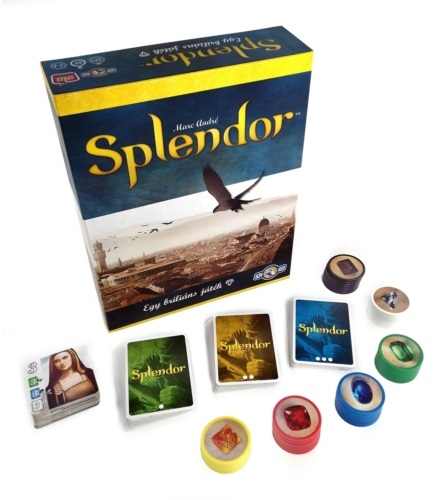
\includegraphics[width=7cm]{images/physical_edition1.jpg}}}$
\hspace{1cm}
$\vcenter{\hbox{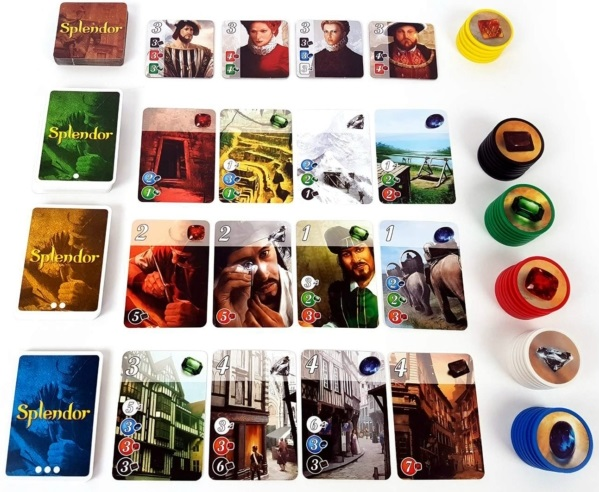
\includegraphics[width=7cm]{images/physical_edition2.jpg}}}$
\caption{A játék fizikális megvalósítása.}
\label{fig:physical}
\end{figure}

\Section{Szoftveres implementációk}

A szoftveres megvalósítása is elkészült a játéknak egy évvel a megjelenése után. Steamen elérhető a kiegészítőivel együtt, természetesen a játék és a kiegészítők megvásárlásával. Korábban telefonokra is elérhető volt, de ma már sajnos nem.

\begin{figure}[h]
\centering
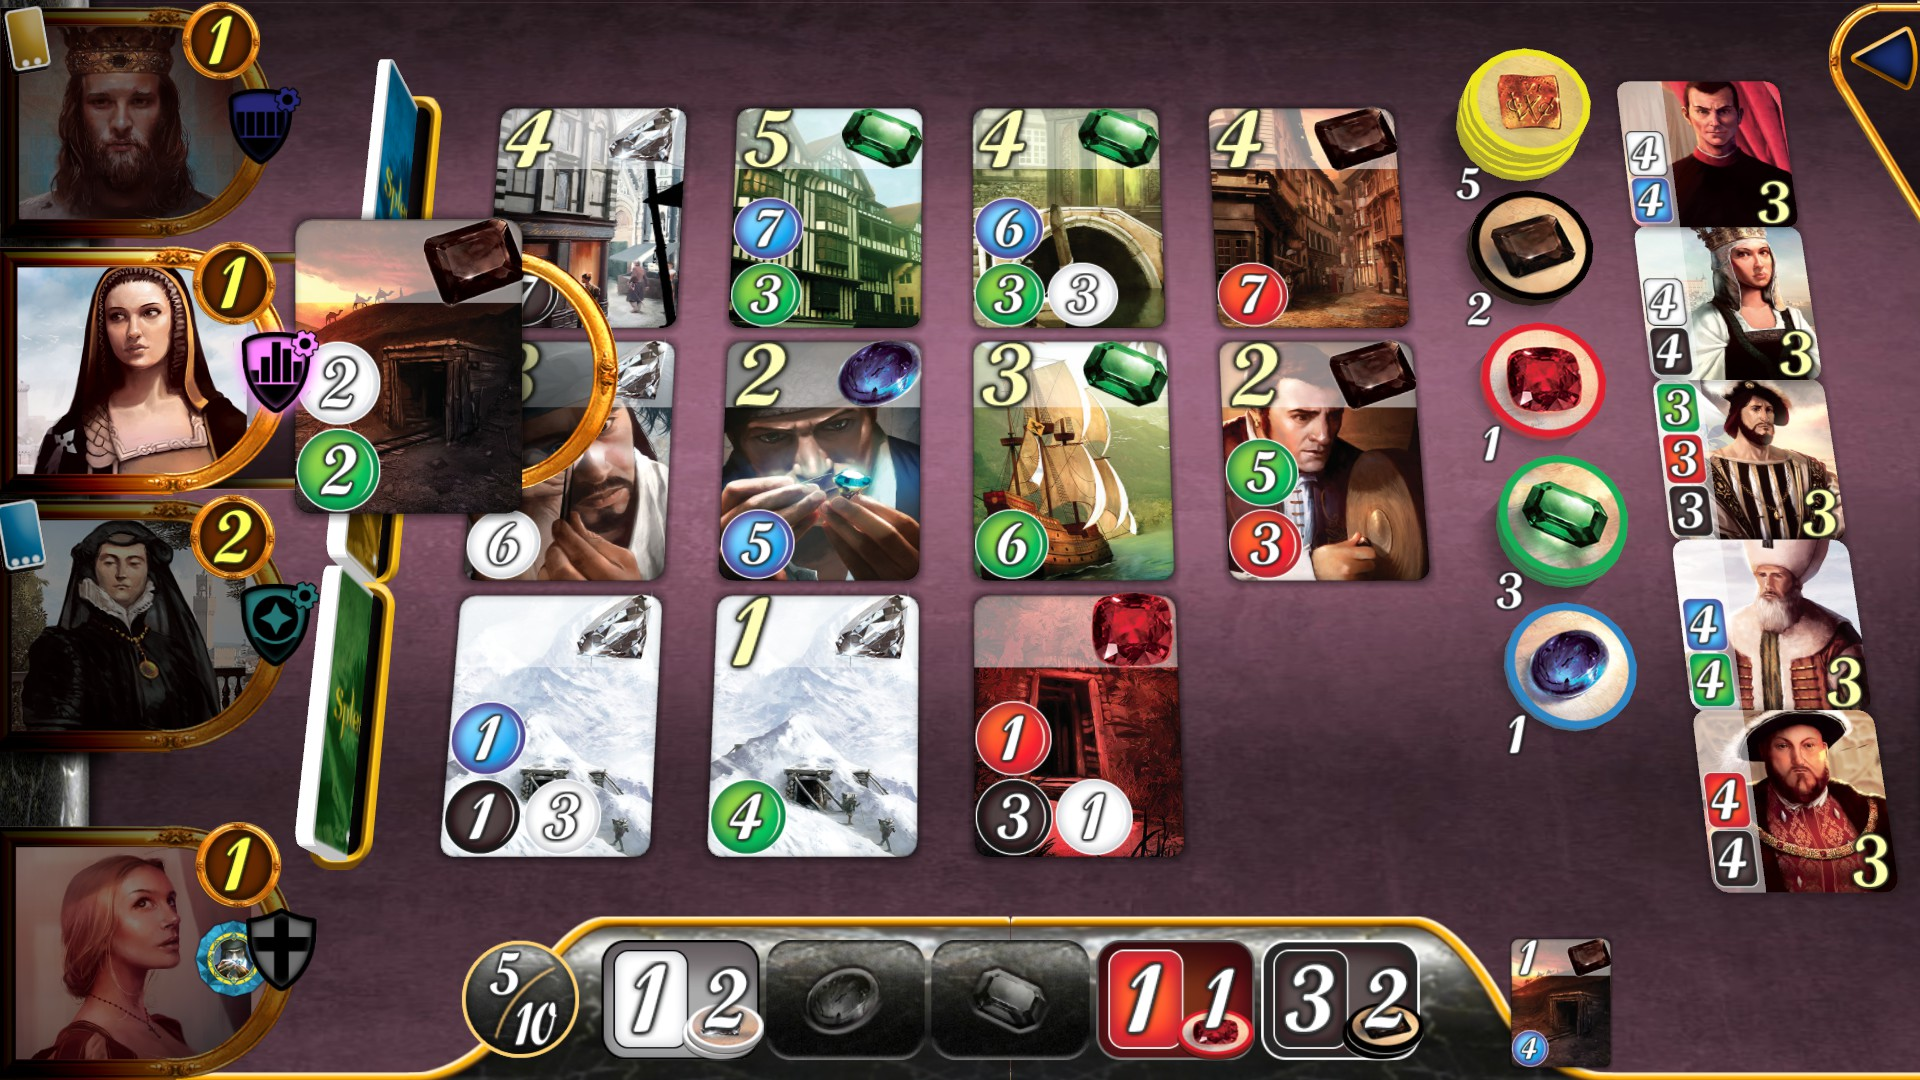
\includegraphics[scale=0.2]{images/digital_edition.jpg}
\caption{A játék szoftveres megvalósítása.}
\label{fig:digital}
\end{figure}